最急降下法では, 直線的に最適解に向かわないので今まで進んできた方向と共役な方向に移動方向を決める方法を共役勾配法という.
\begin{center}
    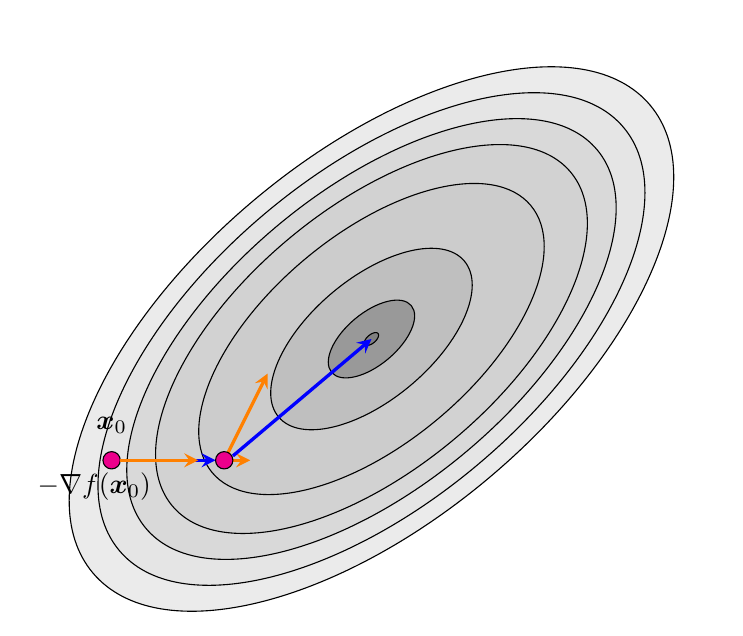
\begin{tikzpicture}[scale=1.1,>=stealth]
        \draw[rotate=40,fill=gray!16,xscale=2] circle[radius=2.1];
        \draw[rotate=40,fill=gray!20,xscale=2] circle[radius=1.9];
        \draw[rotate=40,fill=gray!30,xscale=2] circle[radius=1.7];
        \draw[rotate=40,fill=gray!35,xscale=2] circle[radius=1.5];
        \draw[rotate=40,fill=gray!40,xscale=2] circle[radius=1.2];
        \draw[rotate=40,fill=gray!50,xscale=2] circle[radius=0.7];
        \draw[rotate=40,fill=gray!80,xscale=2] circle[radius=0.3];
        \draw[rotate=40,fill=gray,xscale=2] circle[radius=0.05];
        \draw[->,very thick,draw=blue] (-2.9,-1.4)--(-1.8,-1.4);

        \draw[->,very thick,draw=orange](-1.7,-1.4)--(-1.2,-0.4);
        \draw[->,very thick,draw=orange](-1.6,-1.4)--(-1.4,-1.4);
        \draw[->,very thick,draw=blue] (-1.6,-1.35)--(0,0);
        \draw[fill=magenta] (-3,-1.4) circle[radius=0.1];
        \draw[fill=magenta] (-1.7,-1.4) circle[radius=0.1];
        \node at(-3.2,-1.7) {$-\nabla f(\mbox{\boldmath $x$}_{0})$};
        \node at(-3,-1) {$\mbox{\boldmath $x$}_{0}$};
        \draw[->,very thick,draw=orange](-2.9,-1.4)--(-2,-1.4);
    \end{tikzpicture}
\end{center}
共役勾配法を式にすると以下のように表すことができる.
\begin{align*}
    \begin{array}{l}
    \mbox{\boldmath $x$}_{k}=\mbox{\boldmath $x$}_{k-1}+c_{k}\mbox{\boldmath $p$}_{k}\\
    \mbox{\boldmath $p$}_{k+1}=-\nabla f(\mbox{\boldmath $x$}_{k})+\alpha_{k}\mbox{\boldmath $p$}_{k}
    \end{array} \tag{3.5}
\end{align*}
共役勾配法は勾配だけでなく, \textcolor{red}{今まで進んできた方向も考慮して}探索の方向を決めることで効率化を図っている. 「今までの進んできた方向の考慮」にあたり, \textcolor{red}{ベクトルの共役}という性質を利用する.\\
共役とは, $\mbox{\boldmath $x$},\ \mbox{\boldmath $y$}$が,
\begin{eqnarray*}
    \mbox{\boldmath $x$}^{T}A\mbox{\boldmath $y$}=\langle \mbox{\boldmath $x$},\mbox{\boldmath $y$}\rangle_{A}=0
\end{eqnarray*}
を満たすことをいう.\\
固有ベクトルによる対称行列の対角化を行う.\ $n$次対称行列$A$は\\
固有ベクトル$\mbox{\boldmath $v$}_{1},\mbox{\boldmath $v$}_{2},\cdots,\mbox{\boldmath $v$}_{n}$を並べて作る行列
\begin{eqnarray*}
    V=\begin{pmatrix}\mbox{\boldmath $v$}_{1}&\mbox{\boldmath $v$}_{2}&\cdots&\mbox{\boldmath $v$}_{n}\end{pmatrix}
\end{eqnarray*}
を用いて
\begin{eqnarray*}
    V^{T}AV &=& \Lambda\\
    \Lambda&=&\begin{pmatrix}\lambda_{1}&&&0\\ & \lambda_{2}&&\\ &&\ddots& \\ 0&&&\lambda_{n}\end{pmatrix}
\end{eqnarray*}
ここで, $\lambda_{1},\lambda_{2},\cdots,\lambda_{n}$は固有値であり, このように対角化することが可能となる.\\
ここで$V^{T}V=VV^{T}=I$であるから
\begin{eqnarray*}
    VV^{T}AVV^{T}=V\Lambda V^{T},\ \ A=V\Lambda V^{T}
\end{eqnarray*}
となる. したがって, 対称行列は固有値を対角要素に持つ行列$\Lambda$と固有ベクトルをならべて作る行列$V$で表すことができる\\
したがって共役な$\mbox{\boldmath $x$}_{1},\mbox{\boldmath $x$}_{2}$ついて
\begin{eqnarray*}
    \mbox{\boldmath $x$}_{1}^{T}A\mbox{\boldmath $x$}_{2}&=&\mbox{\boldmath $x$}_{1}^{T}V\Lambda V^{T}\mbox{\boldmath $x$}_{2}\\
                                                        &=&\mbox{\boldmath $x$}_{1}^{T}V\Lambda^{\frac{1}{2}}\Lambda^{\frac{1}{2}}V^{T}\mbox{\boldmath $x$}_{2}\\
                                                        &=&\mbox{\boldmath $x$}_{1}^{T}V\Lambda^{\frac{1}{2}T}\Lambda^{\frac{1}{2}}V^{T}\mbox{\boldmath $x$}_{2}\\
                                                        &=&\mbox{\boldmath $x$}_{1}^{T}\left(\Lambda^{\frac{1}{2}}V^{T}\right)^{T}\Lambda^{\frac{1}{2}}V^{T}\mbox{\boldmath $x$}_{2}\\
    &=&\left(\Lambda^{\frac{1}{2}}V^{T}\mbox{\boldmath $x$}_{1}\right)^{T}\Lambda^{\frac{1}{2}}V^{T}\mbox{\boldmath $x$}_{2}
\end{eqnarray*}
$\Lambda$は対角行列であるのでその平方根である$\Lambda^{\frac{1}{2}}$も対角行列となる. また対角行列の転置行列は元の行列と等しいことを考慮して先のように変形することが出来る.\ ここでベクトル$z$に対して
\begin{eqnarray*}
    \mbox{\boldmath $z$}=\Lambda^{\frac{1}{2}}V^{T}\mbox{\boldmath $x$}
\end{eqnarray*}
なる座標変換をした後のベクトルについて考える.\\
\begin{eqnarray*}
    \mbox{\boldmath $z$}&=&\Lambda^{\frac{1}{2}}V^{T}\mbox{\boldmath $x$}\\
    \mbox{\boldmath $z$}&=&\Lambda^{\frac{1}{2}}\mbox{\boldmath $y$}\\
    \mbox{\boldmath $y$}&=&V^{T}\mbox{\boldmath $x$}
\end{eqnarray*}
とする. そして以下の平面について考える.
\begin{center}
    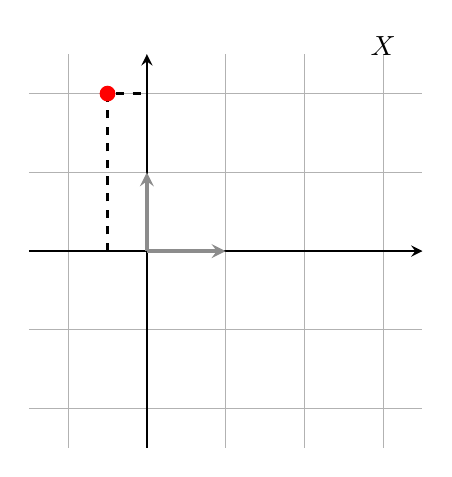
\begin{tikzpicture}[>=stealth]
        \draw[draw=gray!60](-1.5,-2.5) grid (3.5,2.5);
        \draw[thick,->](-1.5,0)--(3.5,0);
        \draw[thick,->](0,-2.5)--(0,2.5);
        \draw[very thick,draw=gray!90,->] (0,0)--(0,1);
        \draw[very thick,draw=gray!90,->] (0,0)--(1,0);
        \draw[dashed,thick](-0.5,0)--(-0.5,2)--(0,2);
        \fill[fill=red] (-0.5,2) circle[radius=0.1];
        \node at(3,2.6) {$X$};
    \end{tikzpicture}
\end{center}
これから$\mbox{\boldmath $y$}$について変換を行うと
\begin{eqnarray*}
    \begin{pmatrix}y_{1}\\y_{2}\end{pmatrix}=\begin{pmatrix}\mbox{\boldmath $v$}_{1}^{T}\mbox{\boldmath $x$}\\\mbox{\boldmath $v$}_{2}^{T}\mbox{\boldmath $x$}\end{pmatrix}
\end{eqnarray*}
となるので$Y$についての平面は以下のように表すことができる.
\begin{center}
    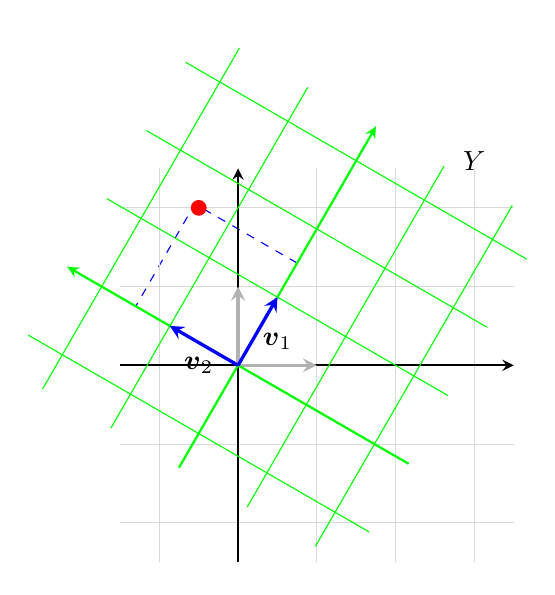
\begin{tikzpicture}[>=stealth]
        \draw[dashed,draw=blue,rotate=60] (1.5,0)--(1.5,1.5)--(0,1.5);
        \draw[draw=gray!30](-1.5,-2.5) grid (3.5,2.5);
        \draw[thick,->](-1.5,0)--(3.5,0);
        \draw[thick,->](0,-2.5)--(0,2.5);
        \draw[very thick,draw=gray!60,->] (0,0)--(0,1);
        \draw[very thick,draw=gray!60,->] (0,0)--(1,0);
        \fill[fill=red] (-0.5,2) circle[radius=0.1];
        \draw[draw=green,rotate=60](-1.5,-2.5) grid (3.5,2.5);
        \draw[thick,->,draw=green,rotate=60](-1.5,0)--(3.5,0);
        \draw[thick,->,draw=green,rotate=60](0,-2.5)--(0,2.5);
        \draw[very thick,draw=blue,->,rotate=60] (0,0)--(0,1);
        \draw[very thick,draw=blue,->,rotate=60] (0,0)--(1,0);

        \node at(3,2.6) {$Y$};
        \node at(0.5,0.3) {$\mbox{\boldmath $v$}_{1}$};
        \node at(-0.5,0) {$\mbox{\boldmath $v$}_{2}$};
    \end{tikzpicture}
\end{center}
これに加えて$\mbox{\boldmath $z$}$に関して,
\begin{eqnarray*}
    \begin{pmatrix}z_{1}\\z_{2}\end{pmatrix}=\begin{pmatrix}\sqrt{\mbox{\boldmath $\lambda$}_{1}}y_{1}\\\sqrt{\mbox{\boldmath $\lambda$}_{1}}y_{1}\end{pmatrix}
\end{eqnarray*}
となるので固有値の平方根をとることで$Z$についての平面は以下のようになる.
\begin{center}
    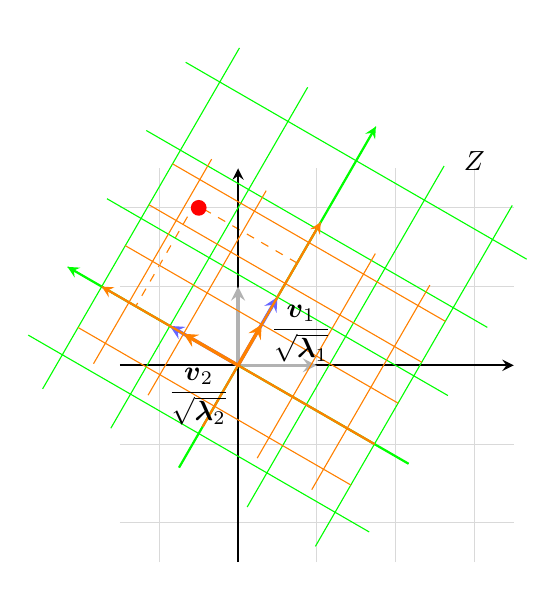
\begin{tikzpicture}[>=stealth]
        \draw[dashed,draw=orange,rotate=60] (1.5,0)--(1.5,1.5)--(0,1.5);
        \draw[draw=gray!30](-1.5,-2.5) grid (3.5,2.5);
        \draw[thick,->](-1.5,0)--(3.5,0);
        \draw[thick,->](0,-2.5)--(0,2.5);
        \draw[very thick,draw=gray!60,->] (0,0)--(0,1);
        \draw[very thick,draw=gray!60,->] (0,0)--(1,0);
        \fill[fill=red] (-0.5,2) circle[radius=0.1];
        \draw[draw=green,rotate=60](-1.5,-2.5) grid (3.5,2.5);
        \draw[thick,->,draw=green,rotate=60](-1.5,0)--(3.5,0);
        \draw[thick,->,draw=green,rotate=60](0,-2.5)--(0,2.5);
        \draw[very thick,draw=blue!60,->,rotate=60] (0,0)--(0,1);
        \draw[very thick,draw=blue!60,->,rotate=60] (0,0)--(1,0);
        \draw[draw=orange,rotate=60,xscale=0.6,yscale=0.8](-1.5,-2.5) grid (3.5,2.5);
        \draw[thick,->,draw=orange,rotate=60,xscale=0.6,yscale=0.8](-1.5,0)--(3.5,0);
        \draw[thick,->,draw=orange,rotate=60,xscale=0.6,yscale=0.8](0,-2.5)--(0,2.5);
        \draw[very thick,draw=orange,->,rotate=60,xscale=0.6,yscale=0.8] (0,0)--(0,1);
        \draw[very thick,draw=orange,->,rotate=60,xscale=0.6,yscale=0.8] (0,0)--(1,0);

        \node at(3,2.6) {$Z$};
        \node at(0.8,0.4) {$\displaystyle \frac{\mbox{\boldmath $v$}_{1}}{\sqrt{\mbox{\boldmath $\lambda$}_{1}}}$};
        \node at(-0.5,-0.4) {$\displaystyle \frac{\mbox{\boldmath $v$}_{2}}{\sqrt{\mbox{\boldmath $\lambda$}_{2}}}$};
    \end{tikzpicture}
\end{center}
座標変換後の直交とは
\begin{eqnarray*}
    \mbox{\boldmath $z$}_{a}^{T}\cdot \mbox{\boldmath $z$}_{b}=0
\end{eqnarray*}
が成立することである.
\begin{center}
    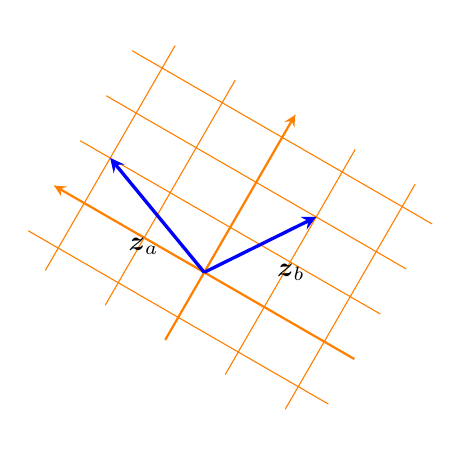
\begin{tikzpicture}[>=stealth,scale=1.1]
        \draw[draw=orange,rotate=60,xscale=0.6,yscale=0.8](-1.5,-2.5) grid (3.5,2.5);
        \draw[thick,->,draw=orange,rotate=60,xscale=0.6,yscale=0.8](-1.5,0)--(3.5,0);
        \draw[thick,->,draw=orange,rotate=60,xscale=0.6,yscale=0.8](0,-2.5)--(0,2.5);
        \draw[rotate=60,very thick,draw=blue,->,xscale=0.6,yscale=0.8] (0,0)--(1,2);
        \draw[rotate=60,very thick,draw=blue,->,xscale=0.6,yscale=0.8] (0,0)--(2,-1);
        \node at(-0.7,0.3) {$\mbox{\boldmath $z$}_{a}$};
        \node at(1,0) {$\mbox{\boldmath $z$}_{b}$};
    \end{tikzpicture}
\end{center}
これについて元の座標においては共役である. つまり
\begin{eqnarray*}
    \mbox{\boldmath $x$}_{a}^{T}A\mbox{\boldmath $x$}_{b}=0
\end{eqnarray*}
ということである.
\begin{center}
    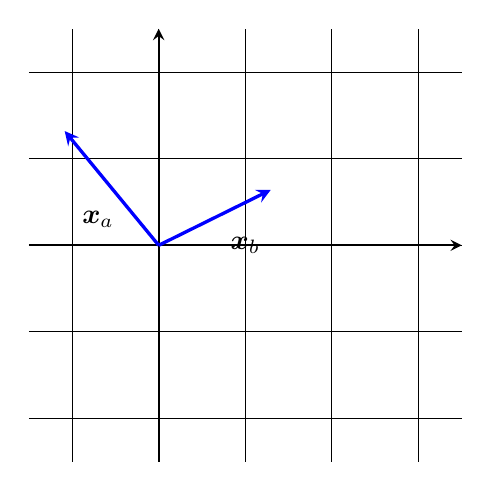
\begin{tikzpicture}[>=stealth,scale=1.1]
        \draw(-1.5,-2.5) grid (3.5,2.5);
        \draw[thick,->](-1.5,0)--(3.5,0);
        \draw[thick,->](0,-2.5)--(0,2.5);
        \draw[rotate=60,very thick,draw=blue,->,xscale=0.6,yscale=0.8] (0,0)--(1,2);
        \draw[rotate=60,very thick,draw=blue,->,xscale=0.6,yscale=0.8] (0,0)--(2,-1);
        \node at(-0.7,0.3) {$\mbox{\boldmath $x$}_{a}$};
        \node at(1,0) {$\mbox{\boldmath $x$}_{b}$};
    \end{tikzpicture}
\end{center}
円については座標変換後の円が
\begin{eqnarray*}
    \mbox{\boldmath $z$}^{T}\cdot \mbox{\boldmath $z$} = {\rm const}
\end{eqnarray*}
とする.
\begin{center}
    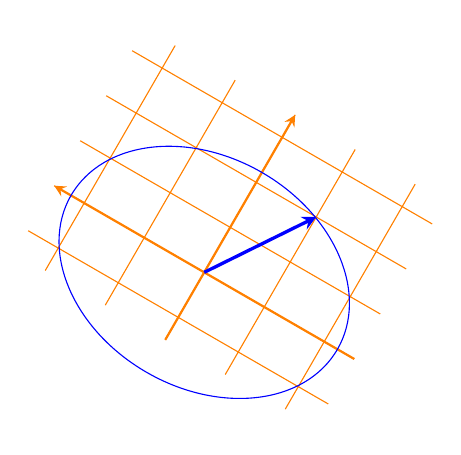
\begin{tikzpicture}[>=stealth,scale=1.1]
        \draw[draw=orange,rotate=60,xscale=0.6,yscale=0.8](-1.5,-2.5) grid (3.5,2.5);
        \draw[thick,->,draw=orange,rotate=60,xscale=0.6,yscale=0.8](-1.5,0)--(3.5,0);
        \draw[thick,->,draw=orange,rotate=60,xscale=0.6,yscale=0.8](0,-2.5)--(0,2.5);
        \draw[rotate=60,very thick,draw=blue,->,xscale=0.6,yscale=0.8] (0,0)--(2,-1);
        \draw[rotate=60,draw=blue,xscale=0.6,yscale=0.8] (0,0) circle[yscale=1.85,xscale=1.85,radius=1.2];
    \end{tikzpicture}
\end{center}
これを元の座標では楕円であり以下の式を満たす
\begin{eqnarray*}
    \mbox{\boldmath $x$}^{T}A\mbox{\boldmath $x$} = {\rm const}
\end{eqnarray*}
このとき半径(長半径, 短半径)は, 固有値の平方根の逆数となる.
\begin{center}
    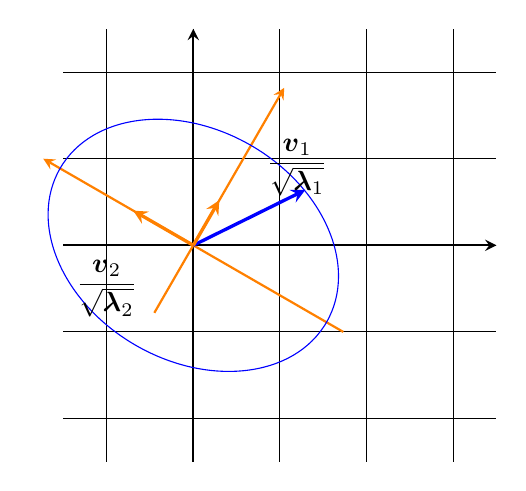
\begin{tikzpicture}[>=stealth,scale=1.1]
        \draw(-1.5,-2.5) grid (3.5,2.5);
        \draw[thick,->](-1.5,0)--(3.5,0);
        \draw[thick,->](0,-2.5)--(0,2.5);
        \draw[thick,->,draw=orange,rotate=60,xscale=0.6,yscale=0.8](-1.5,0)--(3.5,0);
        \draw[thick,->,draw=orange,rotate=60,xscale=0.6,yscale=0.8](0,-2.5)--(0,2.5);
        \draw[rotate=60,very thick,draw=blue,->,xscale=0.6,yscale=0.8] (0,0)--(2,-1);
        \draw[rotate=60,draw=blue,xscale=0.6,yscale=0.8] (0,0) circle[yscale=1.85,xscale=1.85,radius=1.2];
        \draw[rotate=60,draw=orange,very thick,->,xscale=0.6,yscale=0.8] (0,0)--(1,0);
        \draw[rotate=60,draw=orange,very thick,->,xscale=0.6,yscale=0.8] (0,0)--(0,1);
        \node at(1.2,0.9) {$\displaystyle \frac{\mbox{\boldmath $v$}_{1}}{\sqrt{\mbox{\boldmath $\lambda$}_{1}}}$};
        \node at(-1,-0.5) {$\displaystyle \frac{\mbox{\boldmath $v$}_{2}}{\sqrt{\mbox{\boldmath $\lambda$}_{2}}}$};
    \end{tikzpicture}
\end{center}
つまり共役の方向に近似解を更新するということは, 楕円を円に変換したときに直行する方向に近似解を更新することに相当する.
\begin{center}
    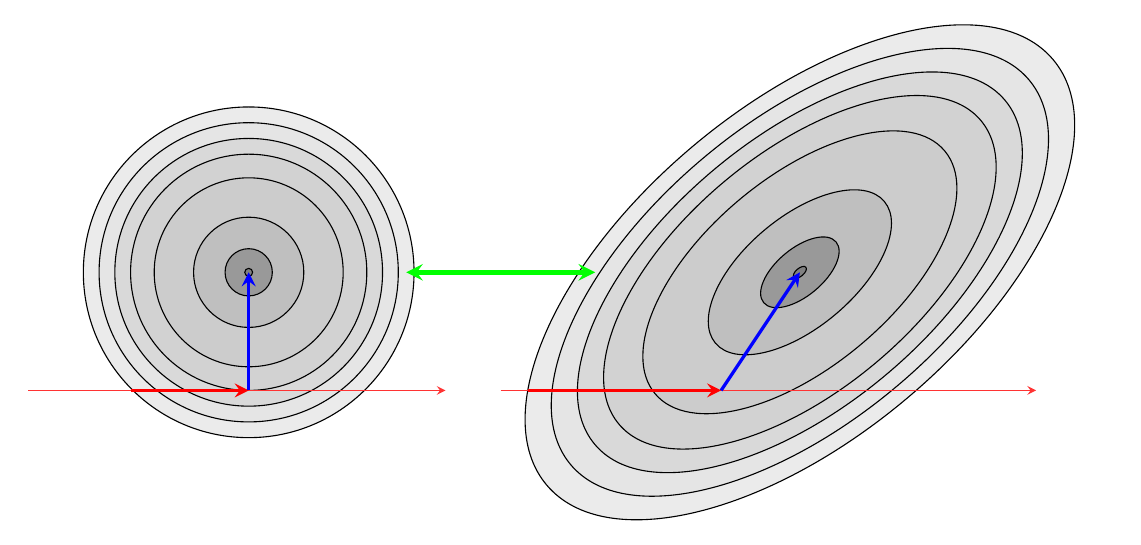
\begin{tikzpicture}[>=stealth]
        \draw[rotate=40,fill=gray!16,xscale=2] (0,0) circle[radius=2.1];
        \draw[rotate=40,fill=gray!20,xscale=2] (0,0) circle[radius=1.9];
        \draw[rotate=40,fill=gray!30,xscale=2] (0,0) circle[radius=1.7];
        \draw[rotate=40,fill=gray!35,xscale=2] (0,0) circle[radius=1.5];
        \draw[rotate=40,fill=gray!40,xscale=2] (0,0) circle[radius=1.2];
        \draw[rotate=40,fill=gray!50,xscale=2] (0,0) circle[radius=0.7];
        \draw[rotate=40,fill=gray!80,xscale=2] (0,0) circle[radius=0.3];
        \draw[rotate=40,fill=gray,xscale=2] (0,0) circle[radius=0.05];

        \draw[fill=gray!16] (-7,0) circle[radius=2.1];
        \draw[fill=gray!20] (-7,0) circle[radius=1.9];
        \draw[fill=gray!30] (-7,0) circle[radius=1.7];
        \draw[fill=gray!35] (-7,0) circle[radius=1.5];
        \draw[fill=gray!40] (-7,0) circle[radius=1.2];
        \draw[fill=gray!50] (-7,0) circle[radius=0.7];
        \draw[fill=gray!80] (-7,0) circle[radius=0.3];
        \draw[fill=gray] (-7,0) circle[radius=0.05];
        \draw[draw=red!80,->] (-9.8,-1.5)--(-4.5,-1.5);
        \draw[draw=red,very thick,->] (-8.5,-1.5)--(-7,-1.5);
        \draw[draw=blue,very thick,->] (-7,-1.5)--(-7,0);
        \draw[draw=red!80,->] (-3.8,-1.5)--(3,-1.5);
        \draw[draw=red,->,very thick] (-3.45,-1.5)--(-1,-1.5);
        \draw[draw=blue,->,very thick] (-1,-1.5)--(0,0);
        \draw[<->,ultra thick,draw=green] (-5,0)--(-2.6,0);
    \end{tikzpicture}
\end{center}
$A$を$N$次正定値対称行列として, 互いな共役なベクトル$\mbox{\boldmath $p$}_{1},\mbox{\boldmath $p$}_{2},\mbox{\boldmath $p$}_{3},\cdots ,\mbox{\boldmath $p$}_{N}$を用いて,
\begin{eqnarray*}
    A\mbox{\boldmath $x$} = \mbox{\boldmath $b$}
\end{eqnarray*}
の解$\mbox{\boldmath $x$}^{*}$を表現することを考える.
\begin{eqnarray*}
    \mbox{\boldmath $x$}^{*}=\sum_{k=1}^{N}c_{k}\mbox{\boldmath $p$}_{k}
\end{eqnarray*}
とおくと, \\
$\mbox{\boldmath $p$}_{i}$は, $\mbox{\boldmath $p$}_{j}\ (j\neq i)$は共役であるから,
\begin{eqnarray*}
    &&\mbox{\boldmath $p$}_{i}^{T}A\mbox{\boldmath $x$}^{*}=\mbox{\boldmath $p$}_{i}^{T}\sum_{k=1}^{N}c_{k}A\mbox{\boldmath $p$}_{k}=c_{i}\mbox{\boldmath $p$}_{i}^{T}A\mbox{\boldmath $p$}_{i}=\mbox{\boldmath $p$}_{i}^{T}\mbox{\boldmath $b$}\\
    \Longrightarrow&&\ c_{i}=\frac{\mbox{\boldmath $p$}_{i}^{T}\mbox{\boldmath $b$}}{\mbox{\boldmath $p$}_{i}^{T}A\mbox{\boldmath $p$}_{i}}
\end{eqnarray*}
として$c_{i}$を定めることができる.\\[0.5cm]
共役勾配法の2次形式の場合の解を求めてみる. つまり
\begin{eqnarray*}
    f(\mbox{\boldmath $x$})=\frac{1}{2}\mbox{\boldmath $x$}^{T}A\mbox{\boldmath $x$}-\mbox{\boldmath $b$}^{T}\mbox{\boldmath $x$}
\end{eqnarray*}
に対して
\begin{eqnarray*}
    \nabla f(\mbox{\boldmath $x$})=A\mbox{\boldmath $x$}-\mbox{\boldmath $b$}=0
\end{eqnarray*}
すなわち
\begin{eqnarray*}
    A\mbox{\boldmath $x$}=\mbox{\boldmath $b$}
\end{eqnarray*}
の解を求める.\\
適当な初期値$\mbox{\boldmath $x$}_{0}$を定め, その負の勾配を$\mbox{\boldmath $r$}_{0}$とする.
\begin{eqnarray*}
    \mbox{\boldmath $r$}_{0}=-\nabla f(\mbox{\boldmath $x$}_{0}+\mbox{\boldmath $b$})
\end{eqnarray*}
最初の基底$\mbox{\boldmath $p$}_{1}$を$\mbox{\boldmath $r$}_{0}$にとる.\ つまり
\begin{eqnarray*}
    \mbox{\boldmath $p$}_{1}=\mbox{\boldmath $r$}_{0}=-A\mbox{\boldmath $x$}_{0}+\mbox{\boldmath $b$}
\end{eqnarray*}
第$k$次の基底$\mbox{\boldmath $p$}_{k}$が定まった時
\begin{eqnarray*}
    c_{k}=\frac{\mbox{\boldmath $p$}_{k}^{T}\mbox{\boldmath $b$}}{\mbox{\boldmath $p$}_{k}^{T}A\mbox{\boldmath $p$}_{k}}
\end{eqnarray*}
を用いて, $\mbox{\boldmath $x$}_{k}$を
\begin{eqnarray*}
    \mbox{\boldmath $x$}_{k}=\mbox{\boldmath $x$}_{k-1}+c_{k}\mbox{\boldmath $p$}_{k}
\end{eqnarray*}
と求められる. これから$\mbox{\boldmath $x$}_{k}$での勾配$\mbox{\boldmath $r$}_{k}$を求めることができる.
\begin{eqnarray*}
    \mbox{\boldmath $r$}_{k}=-\nabla f(\mbox{\boldmath $x$}_{k})=-A\mbox{\boldmath $x$}_{k}+\mbox{\boldmath $b$}
\end{eqnarray*}
第$k+1$次の基底$\mbox{\boldmath $p$}_{k+1}$を, $\mbox{\boldmath $r$}_{k}$と$\mbox{\boldmath $p$}_{k}$の合成, つまり
\begin{eqnarray*}
    \mbox{\boldmath $p$}_{k+1}=\mbox{\boldmath $r$}_{k}+\alpha_{k}\mbox{\boldmath $p$}_{k}
\end{eqnarray*}
とおいて, これが$\mbox{\boldmath $p$}_{k}$と共役となるように定める.\\
このとき, $\alpha_{k}$は以下の等式を満たす.
\begin{eqnarray*}
    \mbox{\boldmath $p$}_{k}^{T}A\mbox{\boldmath $p$}_{k+1}=\mbox{\boldmath $p$}_{k}^{T}A(\mbox{\boldmath $r$}_{k}+\alpha_{k}\mbox{\boldmath $p$}_{k})=\mbox{\boldmath $p$}_{k}^{T}A\mbox{\boldmath $r$}_{k}+\alpha_{k}\mbox{\boldmath $p$}_{k}^{T}\mbox{\boldmath $p$}_{k}=0
\end{eqnarray*}
したがって
\begin{eqnarray*}
    \alpha_{k}=-\frac{\mbox{\boldmath $p$}_{k}^{T}A\mbox{\boldmath $r$}_{k}}{\mbox{\boldmath $p$}_{k}^{T}A\mbox{\boldmath $p$}_{k}}
\end{eqnarray*}
よって, 求める第$k+1$次の基底は
\begin{eqnarray*}
    \mbox{\boldmath $p$}_{k+1}=\mbox{\boldmath $r$}_{k}+\alpha_{k}\mbox{\boldmath $p$}_{k}=\mbox{\boldmath $r$}_{k}-\frac{\mbox{\boldmath $p$}_{k}^{T}A\mbox{\boldmath $r$}_{k}}{\mbox{\boldmath $p$}_{k}^{T}A\mbox{\boldmath $p$}_{k}}\mbox{\boldmath $p$}_{k}
\end{eqnarray*}
と求まる. さらに, これを用いて$\mbox{\boldmath $x$}_{k+1}$を
\begin{eqnarray*}
    c_{k+1}&=&\frac{\mbox{\boldmath $p$}_{k+1}^{T}\mbox{\boldmath $b$}}{\mbox{\boldmath $p$}_{k+1}^{T}A\mbox{\boldmath $p$}_{k+1}}\\
    \mbox{\boldmath $x$}_{k+1}&=&\mbox{\boldmath $x$}_{k}+c_{k+1}\mbox{\boldmath $p$}_{k+1}
\end{eqnarray*}
と求まる.\\
これより関数が2次形式であれば, くりかえし回数は, たかだか共役なベクトルの数(つまり$\mbox{\boldmath $x$}$の次元数)となる.
